\section{Overview}
From earlier calibration versions of data from the autocorrelators
of Odin-SMR we know that calibrated spectra from both high and 
low altitudes contain spectral features not caused by the atmospheric
species.
This short report contains a likely explanation
of how these spectral features are induced
and how they affect the spectra.


\clearpage
\newpage

\section{Spectral features in spectra}
\begin{figure}[!t]
\centering
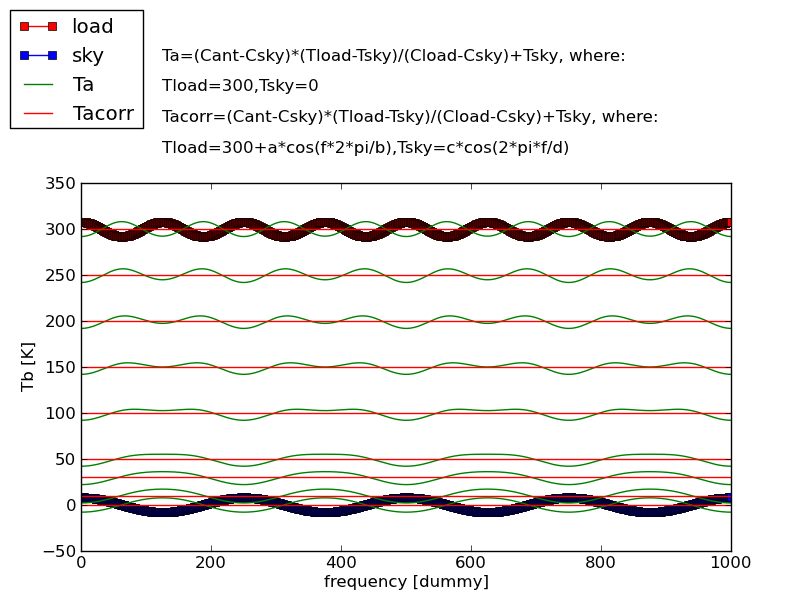
\includegraphics[scale=0.7]{odinspectrumpattern.png}\\
\caption{Wave induced pattern in calibrated spectra. The red line represents 
a perturbed brightness temperature spectrum of the
hot load (a cosinus wave with eight cycles is added)
The blue line represents a perturbed brightness temperature
spectrum of the cold sky (a cosinus wave with four cycles is added).
The thin red lines represent perfectly calibrated spectra.
The green lines show what features the cosinus waves of the
references induce on calibrated spectra if they are not taken into account.
}
\label{fig:study2ac2a}
\end{figure}

From earlier calibration versions of data from the autocorrelators
of Odin-SMR we know that calibrated spectra from both high and 
low altitudes contain spectral features not caused by the atmospheric
species. 
The spectral features, which are different at low and and high altitudes, 
are instead caused by the instrument itself and not taken into account
in the calibration process.

The calibration process (level1a to level1b) is based on that we have 
measurements of the clod sky (\(C_{s}(f)\) at 2.7 K), hot load (\(C_{L}(f)\)
at around 290 K), and the target atmosphere (\(C_{A}(f)\) 
at unkown temperature \(T_{A}\)).
The calibration process can be understand as a linear interpolation
of \(C_{A}(f)\)  using \(C_{s}(f)\) and \(C_{L}(f)\) and their temperatures
as references.
 
The calibration process assumes that both the cold sky and hot load signal
are clean. Figure~\ref{fig:study2ac2a} shows an example of what would happen with
calibrated spectra if these signals are not clean
(but the target signal is clean).
In the example the blue line represents a perturbed brightness temperature
spectrum of the cold sky (a cosinus wave with four cycles is added).
The red line represents a perturbed brightness temperature spectrum of the
hot load (a cosinus wave with eight cycles is added).
The thin red lines can be interpreted as perfectly calibrated spectra.

The green lines show what features the cosinus waves of the
references induce on calibrated spectra if they are not taken into account:

At low brightness temperatures this pattern is caused by the
the wave on the cold sky signal (and 180 degree phase shifted
w.r.t. wave on the cold sky signal).

At high brightness temperatures this pattern is caused by the
the wave on the hot load signal (and 180 degree phase shifted
w.r.t. wave on the hot load signal).

At intermediate brightness temperatures the pattern is a linear
combination of the mentioned pattern,
i.e. (using the equations in the figure) 
\begin{equation}
\Delta T=c \cdot cos\left(\frac{f2\pi}{d}+\pi\right) \cdot (1-w(f)) 
+a \cdot cos \left( \frac{f2\pi}{b}+\pi \right) \cdot w(f)
\end{equation}
where
\begin{equation}
w(f)=\frac{C_{A}(f)-C_{s}(f)}{C_{L}(f)-C_{S}(f)}\approx\frac{T_{A}(f)}{T_{L}(f)}
\end{equation}

\section{Odin data}
\subsection{AC2}
\begin{figure}[!t]
\centering
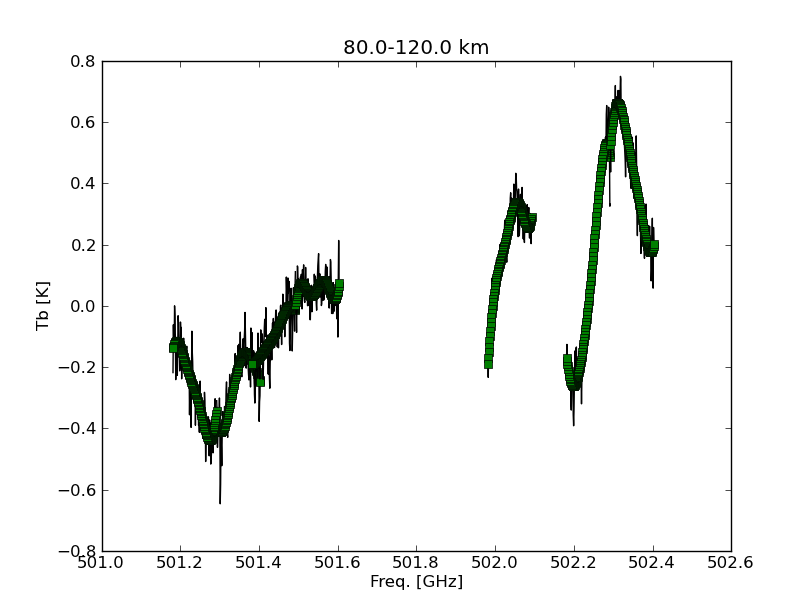
\includegraphics[scale=0.7]{ac2spechigh.png}\\
\caption{High tangent altitude median spectrum from AC2 (strat 1).}
\label{fig:study2spec1}
\end{figure}

\begin{figure}[!t]
\centering
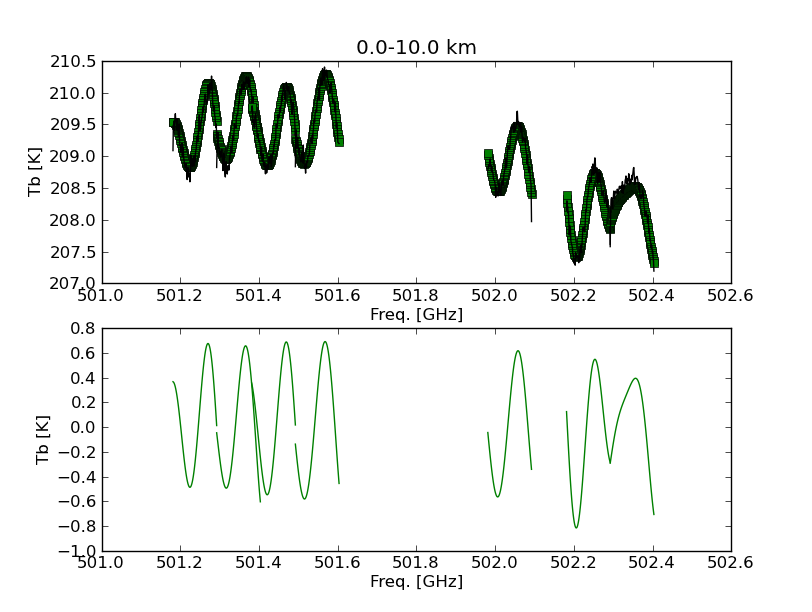
\includegraphics[scale=0.7]{ac2speclow.png}\\
\caption{Low tangent altitude median spectrum from AC2 (strat 1).}
\label{fig:study2spec2}
\end{figure}

\begin{figure}[!t]
\centering
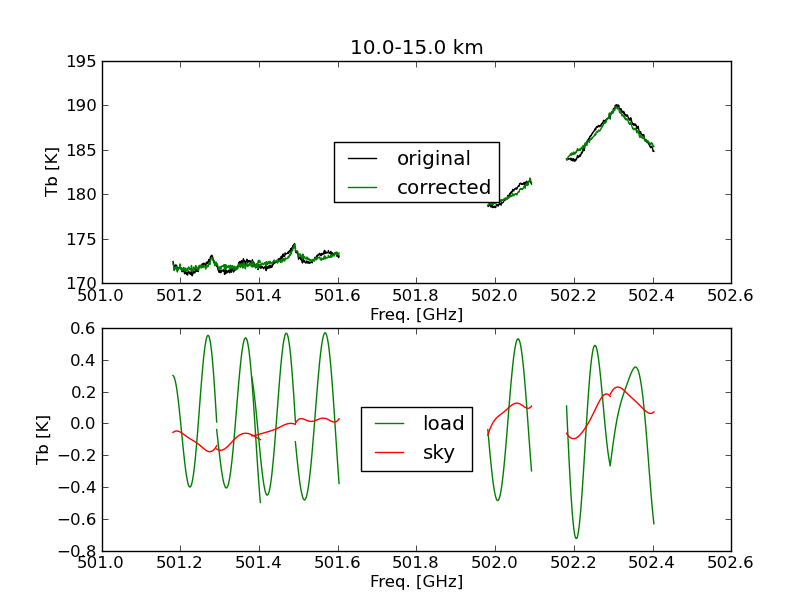
\includegraphics[scale=0.7]{ac2spec1015.png}\\
\caption{Intermediate tangent altitude median spectrum from AC2 (strat 1).}
\label{fig:study2spec3}
\end{figure}

\begin{figure}[!t]
\centering
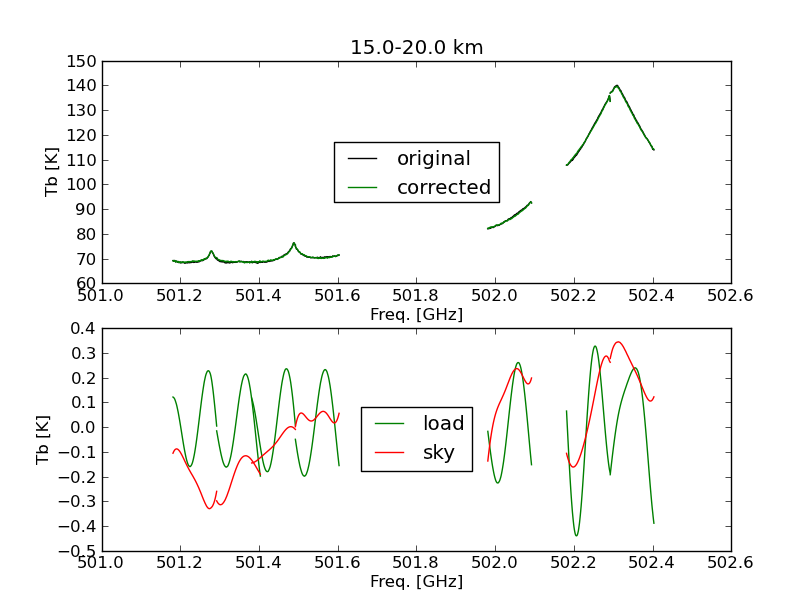
\includegraphics[scale=0.7]{ac2spec1520.png}\\
\caption{Intermediate tangent altitude median spectrum from AC2 (strat 1).}
\label{fig:study2spec4}
\end{figure}

\begin{figure}[!t]
\centering
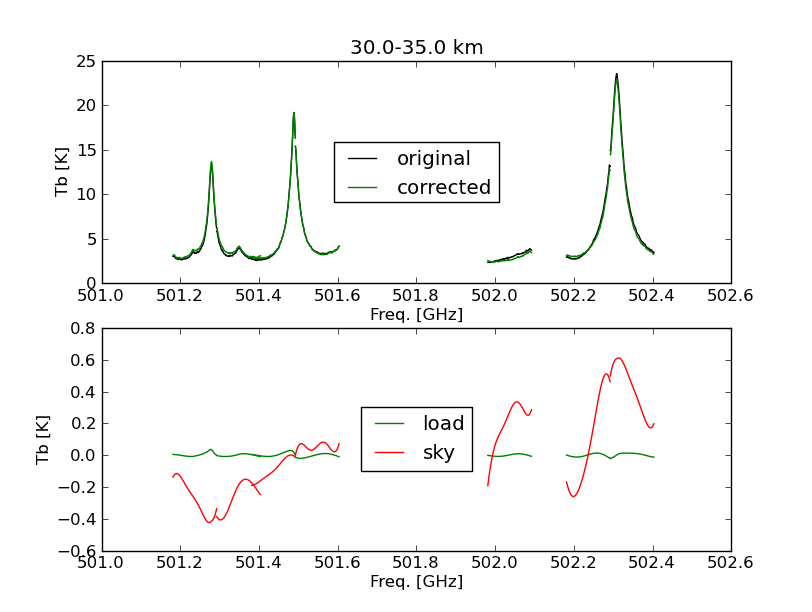
\includegraphics[scale=0.7]{ac2spec3035.png}\\
\caption{Intermediate tangent altitude median spectrum from AC2 (strat 1).}
\label{fig:study2spec5}
\end{figure}

\begin{figure}[!t]
\centering
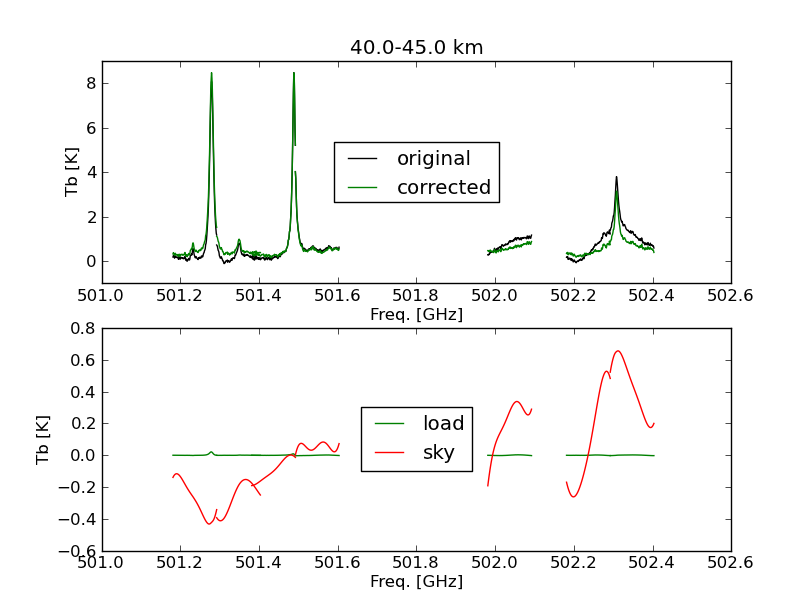
\includegraphics[scale=0.7]{ac2spec4045.png}\\
\caption{Intermediate tangent altitude median spectrum from AC2 (strat 1).}
\label{fig:study2spec6}
\end{figure}

\begin{figure}[!t]
\centering
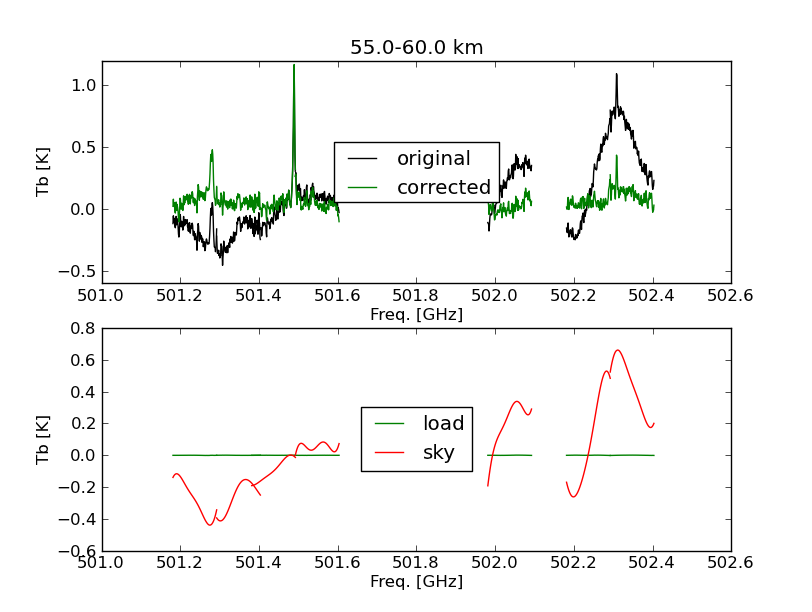
\includegraphics[scale=0.7]{ac2spec5560.png}\\
\caption{Intermediate tangent altitude median spectrum from AC2 (strat 1).}
\label{fig:study2spec7}
\end{figure}
\clearpage
\newpage
\subsection{AC1}
\begin{figure}[!t]
\centering
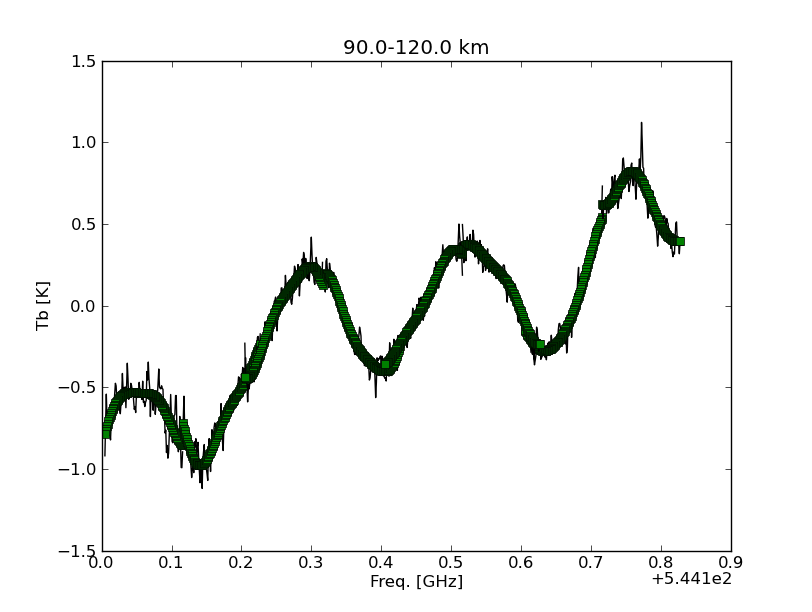
\includegraphics[scale=0.7]{ac1spechigh.png}\\
\caption{High tangent altitude median spectrum from AC1 (strat 2).}
\label{fig:study2spec8}
\end{figure}

\begin{figure}[!t]
\centering
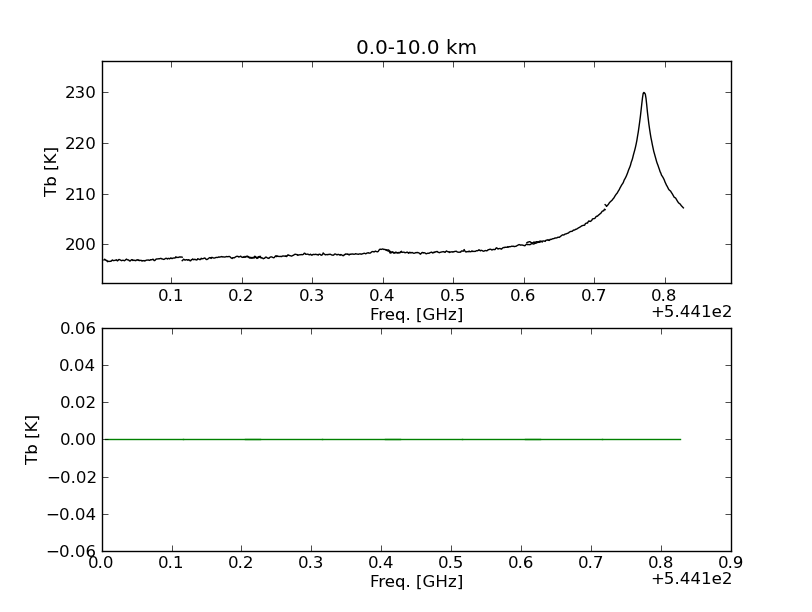
\includegraphics[scale=0.7]{ac1speclow.png}\\
\caption{Low tangent altitude median spectrum from AC1 (strat 2).}
\label{fig:study2spec9}
\end{figure}



\begin{figure}[!t]
\centering
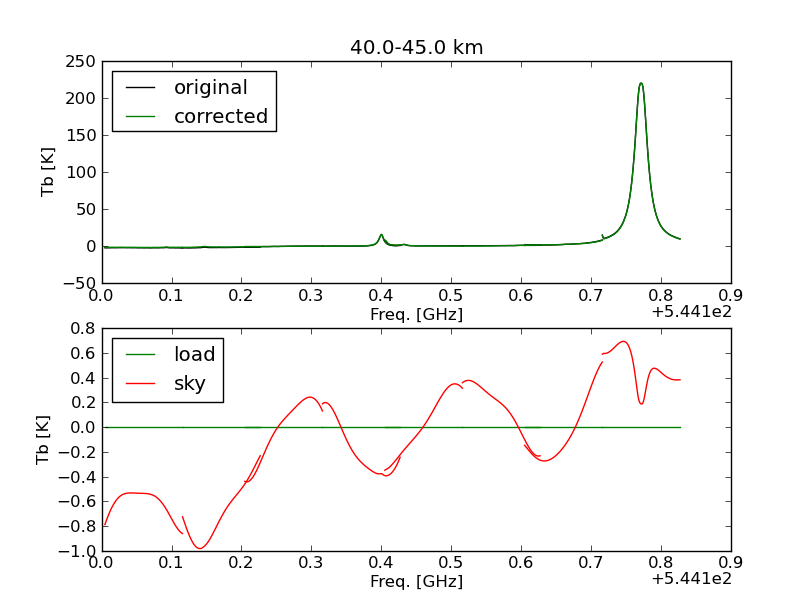
\includegraphics[scale=0.7]{ac1spec4045.png}\\
\caption{Intermediate tangent altitude median spectrum from AC1 (strat 2).}
\label{fig:spec1}
\end{figure}

\begin{figure}[!t]
\centering
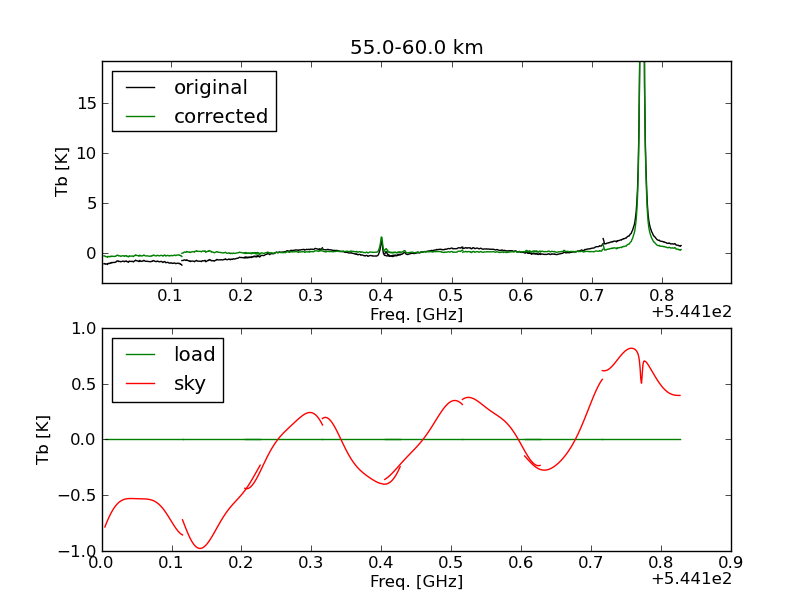
\includegraphics[scale=0.7]{ac1spec5560.png}\\
\caption{Intermediate tangent altitude median spectrum from AC1 (strat 2).}
\label{fig:spec1}
\end{figure}





